%در این قسمت نحوه استفاده از doxygen و doxywizard آورده شده است. این بخش شامل دو زیر بخش خواهد بود
%یکی نحوه استفاده از doxygen به صورت خط فرمان و دیگری استفاده از doxygen به صورت گرافیکی که همان
%استفاده از doxywizard است.
%محمد هادی منصوری ۹۰/۳/۲۰
%\section {
%%نحوه‌ی استفاده از {\lr{Doxygen}} و {\{Doxywizard}}
%نحوه‌ی استفاده از Doxygen و Doxywizard
%}
در این قسمت  نحوه‌ی استفاده از \lr{Doxygen} و \lr{Doxywizard} توضیح داده شده است. 
برنامه‌ی اجرایی \lr{Doxygen} در واقع ابزار اصلی برای تولید مستند است. این برنامه پرونده‌های منبع\footnote{\lr{Source Files}} را تجزیه\footnote{\lr{Parse}}
 کرده و مستند مورد نظر را از پرونده‌های منبع تولید می‌کند. لازم به ذکر است که مستندات در پرونده‌های منبع باید 
به شکلی خاص نوشته شود، که نحوه‌ی نوشتن مستندات در پرونده‌های منبع در فصل‌های آتی توضیح داده شده است.

\lr{Doxygen} 
از یک پرونده‌ی پیکربندی\footnote{\lr{Configuration File}}
 برای تولید مستند استفاده می کند. در این پرونده‌ی پیکربندی، تنظیمات مربوط به نحوه‌ی تولید مستند، 
نوع پرونده‌های ورودی و خروجی، ظاهر مستند تولیدی و سایر تنظیمات قرار داده می‌شود. با ویرایش پرونده‌ی پیکربندی می‌توانیم تنظیمات 
دلخواه خود را برای \lr{Doxygen} تعیین کنیم.

\lr{Doxygen} 
اساسا یک ابزار کاربردی بر مبنای خط فرمان\footnote{\lr{Command Line}} 
است. بنابراین برای اجرا و استفاده از آن باید از طریق خط فرمان دستورات لازم را بدهیم. اما برخی ابزارهای گرافیکی وجود دارند 
که با استفاده از آن‌ها می‌توانیم \lr{Doxygen} را به صورت گرافیکی مورد استفاده قرار دهیم و نیازی به وارد کردن دستورات از طریق 
خط فرمان نیست. \lr{Doxywizard} یکی از این برنامه‌های گرافیکی است. با استفاده از \lr{Doxywizard} می‌توان یک پرونده‌ی پیکربندی 
ایجاد کرد یا یک پرونده‌ی پیکربندی را ویرایش کرد. همچنین با استفاده از این برنامه می‌توان \lr{Doxygen} را 
بدون نیاز به دستورات خط فرمان اجرا کرد. در تصویر \ref{doxygen_doxywizard} ارتباط  \lr{Doxygen} و \lr{Doxywizard}، به صورت 
ساده نشان داده شده است.
\begin{figure}
  \centering
  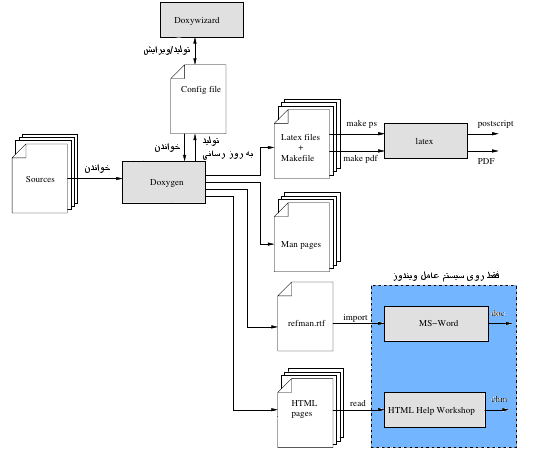
\includegraphics[width=0.75\textwidth]{image/doxygen_doxywizard}
  \caption[ارتباط \lr{Doxygen} و \lr{Doxywizard}.]{
ارتباط \lr{Doxygen} و \lr{Doxywizard}.
\lr{Doxygen} 
برنامه‌ی اصلی برای تولید مستند از پرونده‌های منبع است که برای تولید نیاز به یک پرونده‌ی پیکربندی دارد. \lr{Doxywizard} ساخت 
پرونده‌ی پیکربندی را برای کاربران ساده می‌کند و به کاربران اجازه می‌دهد پرونده‌های پیکربندی را ویرایش کنند. همچنین از طریق آن 
می‌توان \lr{Doxygen} را اجرا کرد.
  }
  \label{doxygen_doxywizard}
\end{figure}

\begin{sloppypar}
\lr{Doxygen} 
 زبان‌های برنامه نویسی بسیاری را حمایت می‌کند. به صورت پیش فرض زبان‌های 
\lr{C}، \lr{C++}، \lr{C\#}، \lr{Objective-C}، \lr{Java}، \lr{PHP}، \lr{Python}، \lr{Fortran}، \lr{IDL}، \lr{VHDL} و \lr{D} 
توسط \lr{Doxygen} حمایت می‌شوند. یعنی اگر پرونده‌هایی که در آن‌ها مستندات و کدهای خود را نوشته‌اید به یکی از این زبان‌ها باشد، 
می توانید با استفاده از \lr{Doxygen}، مستند فنی آن‌ها را تولید کنید. 
البته تجزیه‌کننده\footnote{\lr{Parser}} و پالایه\footnote{\lr{Filter}} برای زبان‌های دیگر نیز توسط افراد یا 
گروه‌های دیگر ساخته شده و یا در حال ساخت است. برای اطلاع از این موارد به آدرس 
\lr{http://www.doxygen.org/helpers.html} 
مراجعه نمایید. \lr{Doxygen} زبان برنامه نویسی نوشته شده در پرونده‌ها را از پسوند پرونده‌ها تشخیص می‌دهد. به عنوان مثال 
اگر پسوند یک پرونده \lr{.f} باشد، \lr{Doxygen} زبان برنامه نویسی نوشته شده در آن پرونده‌را زبان فرترن در نظر می‌گیرد، 
یا اگر پسوند پرونده‌ای \lr{.java} باشد، زبان برنامه نویسی آن پرونده زبان جاوا در نظر گرفته می‌شود. البته می‌توان با 
ویرایش پرونده‌ی پیکربندی، این نوع تشخیص را عوض کرد.
\end{sloppypar}

با استفاده از \lr{Doxygen}  می‌توان مستندات را در قالب‌های مختلفی تولید کرد. قالب‌های 
\lr{HTML}، \lr{LaTeX}، \lr{Man pages}، \lr{RTF}، \lr{XML} و \lr{Qt Help Project (.qhp)} 
در \lr{Doxygen} به صورت مستقیم حمایت می‌شوند، و قالب‌های 
\lr{Qt Compressed Help (.qhc)}، \lr{PostScript (.ps)} و \lr{PDF} 
نیز به طور غیر مستقیم حمایت می‌شوند، به این ترتیب که مستندات در قالب \lr{.qhc} را می‌توان از طریق مستندات 
تولید شده در قالب \lr{.qhp} ساخت و مستندات در قالب \lr{PostScript} و \lr{PDF} را هم می‌توان از طریق مستندات 
تولید شده در قالب \lr{LateX} به دست آورد.


در این فصل، در قسمت اول کار با \lr{Doxygen} از طریق خط فرمان را شرح می‌دهیم و در قسمت بعد، نحوه‌ی استفاده از \lr{Doxywizard} را 
بیان می‌کنیم که یک واسط گرافیکی برای استفاده از \lr{Doxygen} است.